% Provenance (never printed): see sources/outline_sources.md (Year 1: the carbonate factory;
% reefs and platforms; pelagic oozes and the carbonate compensation depth; siliceous oozes;
% evaporite sequences). Exercise and problem values in the Book 3 scratch calculator
% calc/ch22.py; figure data from figdata/bachelor-1/evaporation.py and ccd_flank.py.
% Calcite, aragonite and dolomite are ch. 7's; the depth--age law ch. 13's; salinity Book 1's
% (g8); limestone Book 1's (g6, prose); the carbonate system and alkalinity the chemistry and
% biology books' (recalled, never defined). The subsidence of volcanic islands under reefs is
% the Year 2 volume's (oceanic islands); diagenesis (dolomitisation, chert, gypsum to
% anhydrite) is ch. 23's; upwelling ch. 29's.
\chapter{Carbonate, Siliceous and Evaporite Sediments}\label{ch:b1:chemical-biogenic-sediments}

The white cliffs of chalk that face each other across the narrow sea between
England and France look like the most ordinary of rocks. Under the electron
microscope they turn out to be made of countless tiny plates of calcite, shed
by single-celled algae that floated in the sea that covered the region. A
\omterm{def:b1:chemical-biogenic-sediments:reef}{reef} seen from a boat is the same story at the other end of the scale: a
limestone in the making, built by corals and algae that take calcium and
carbonate from the water and turn them into stone. Not all sediments are
carried; many are made where they lie, by living things or by the water itself
as it evaporates. This chapter follows the three great families of these
sediments --- carbonates, \omterm{def:b1:chemical-biogenic-sediments:ooze}{siliceous oozes} and \omterm{def:b1:chemical-biogenic-sediments:evaporite}{evaporites} --- from the
chemistry of the sea that feeds them to the rocks they leave.

\begin{recall}
Limestone is a sedimentary rock made of calcite, often from shells, and it
fizzes in dilute acid (Book~1, grade~6). Calcite and aragonite are the two
\omterm{def:b1:rock-forming-minerals:polymorph}{polymorphs} of \ce{CaCO3}, of densities \qty{2.71}{g.cm^{-3}} and
\qty{2.93}{g.cm^{-3}}, and dolomite \ce{CaMg(CO3)2}, of density
\qty{2.84}{g.cm^{-3}}, is the carbonate of calcium and magnesium
(\cref{ch:b1:rock-forming-minerals}). The salinity of seawater is the mass of
salt dissolved in a kilogram of it (Book~1, grade~8). In water, carbon dioxide,
hydrogen carbonate and carbonate ions are linked by acid--base equilibria, and
the alkalinity measures the bases able to take up hydrogen ions (the chemistry
books); the ocean's carbonate system takes part in the carbon cycle (the biology
books). The sea floor deepens with age as $d = d_r + C\sqrt t$
(\cref{thm:b1:rifts-ridges-margins:depth-age}).
\end{recall}
% ledger: webmineral:polymorphs, hom:calcite, webmineral:others

\section{The carbonate factory}\label{sec:b1:chemical-biogenic-sediments:factory}

Seawater holds calcium and dissolved inorganic carbon, mostly as hydrogen
carbonate. Calcium carbonate forms from them by the reactions
\[
\ce{Ca^2+ + 2 HCO3- -> CaCO3 + CO2 + H2O}, \qquad
\ce{Ca^2+ + CO3^2- -> CaCO3},
\]
the first releasing a molecule of carbon dioxide for each one of carbonate
laid down. Warm surface water of the tropics is supersaturated in calcium
carbonate, but it seldom precipitates by itself: almost all of it is made by
living things, which pay the energy to build their shells and skeletons and
control the \omterm{def:b1:rock-forming-minerals:mineral}{mineral} they use. Corals and green algae build aragonite; red
algae and many foraminifera build calcite, some of it rich in magnesium;
molluscs use one or both.

\begin{definition}[Carbonate factory]\label{def:b1:chemical-biogenic-sediments:factory}
The \emph{carbonate factory}\index{carbonate factory} of a sea is the set of
organisms and processes that produce calcium carbonate sediment where it is
found, rather than bringing it from elsewhere. Its products are skeletal grains
(whole or broken shells and skeletons), carbonate mud, coated grains and the
rigid frameworks of \omterm{def:b1:chemical-biogenic-sediments:reef}{reefs}.
\end{definition}

The richest factory works in warm, clear, shallow and sunlit water, far from
the mud of rivers, which would bury the producers and cloud the light the
algae need. Its sediment is made by the sea floor itself: coral and algal
debris, the shells of molluscs and of the single-celled foraminifera that live
on the bottom, and needles of aragonite shed by green algae, which settle as a
lime mud. Where the water is agitated and supersaturated, grains rolled about by
the waves and tides grow coats of carbonate, layer on layer, around a nucleus,
a sand grain or a fragment of shell, into round \omterm{def:b1:chemical-biogenic-sediments:reef}{ooids}
(\cref{def:b1:chemical-biogenic-sediments:reef}). A second factory works in the
open ocean, far from any shore: the plankton that live in the sunlit surface
layer build tiny calcite shells and plates that rain down to the deep sea floor
(\cref{sec:b1:chemical-biogenic-sediments:oozes}).
% ledger: og:carbonates

How fast a factory builds is measured by its carbonate budget, the mass of
carbonate produced and kept in place each year on a square metre, after the
losses to boring organisms, grazers and the waves. It turns into a vertical
rate of growth by a mass balance.

\begin{proposition}[Accretion from a carbonate budget]\label{prop:b1:chemical-biogenic-sediments:accretion}
Let a sea floor keep in place the net mass $G$ of calcium carbonate per unit area
and per unit time, as a deposit whose solid grains have the density $\rho_s$
and whose porosity, the fraction of its volume taken by pores, is $\phi$. Then
the floor rises at the rate
\[
a = \frac{G}{\rho_s\,(1-\phi)}.
\]
\end{proposition}

\begin{proof}
In the time $\mathrm dt$ a unit area receives the mass $G\,\mathrm dt$ of
solid carbonate, which fills the volume $G\,\mathrm dt/\rho_s$ of grains. These
grains make up the fraction $1-\phi$ of the new layer, whose thickness is
therefore $G\,\mathrm dt/(\rho_s(1-\phi))$. Dividing by $\mathrm dt$ gives $a$.
\end{proof}

The product $\rho_s(1-\phi)$ is the dry bulk density of the deposit. On the
\omterm{def:b1:chemical-biogenic-sediments:reef}{reefs} of the Chagos Archipelago in the Indian Ocean, 28 \omterm{def:b1:chemical-biogenic-sediments:reef}{reefs} measured in 2015
had an average budget of \qty{3.7}{kg} of \ce{CaCO3} per square metre and per
year, and those dominated by branching \emph{Acropora} corals \qty{8.4}{kg},
growing at about \qty{4.2}{mm} a year; with the proposition, these two numbers
together mean a dry bulk density of \qty{2000}{kg.m^{-3}}, that is a \omterm{def:b1:chemical-biogenic-sediments:reef}{reef}
framework about a third pore space (\cref{exo:b1:chemical-biogenic-sediments:3}).
The same \omterm{def:b1:chemical-biogenic-sediments:reef}{reefs} had lost more than nine tenths of their corals in the warming
event of 1998, and their budgets show how fast a \omterm{def:b1:chemical-biogenic-sediments:reef}{reef} can rebuild.
% ledger: perry:chagos

\section{Reefs and platforms}\label{sec:b1:chemical-biogenic-sediments:reefs}

Where the factory builds a rigid framework, it can stand up from the sea floor
against the waves.

\begin{definition}[Reef, carbonate platform, ooid]\label{def:b1:chemical-biogenic-sediments:reef}
A \emph{reef}\index{reef} is a carbonate build-up whose framework of organisms,
corals, algae or others, grown in place and bound and cemented together, stands
above the surrounding sea floor and resists the waves. A \emph{carbonate
platform}\index{carbonate platform} is a thick body of shallow-water carbonate
whose flat top lies close to sea level and which is bounded by a slope down to
deeper water. An \emph{ooid}\index{ooid} is a round grain of sand size made of
concentric layers of calcium carbonate grown around a nucleus as it rolled in
agitated water; a rock made of ooids is an oolite.
\end{definition}
% ledger: og:carbonates

Modern coral \omterm{def:b1:chemical-biogenic-sediments:reef}{reefs} come in three kinds, named by the voyagers who mapped them
long before anyone drilled through one. A \emph{fringing} \omterm{def:b1:chemical-biogenic-sediments:reef}{reef} is attached to
the shore of an island or a continent. A \emph{barrier} \omterm{def:b1:chemical-biogenic-sediments:reef}{reef} is separated from
the land by a lagoon, which can be wide and tens of metres deep: the barrier
off north-eastern Australia runs, with breaks, for nearly a thousand miles,
enclosing a sea 10 to 25 fathoms deep, about 18 to \qty{46}{m}. An
\emph{atoll} is a ring of \omterm{def:b1:chemical-biogenic-sediments:reef}{reef}, bearing low islands of coral sand, around a
lagoon with no land in it at all.

\begin{omfigure}
\begin{tikzpicture}[font=\footnotesize, scale=0.72]
% three reef types in cross-section (schematic): a volcanic cone y = 2 - s - 0.75|x - 4|
% subsided by s (0, 0.8, 1.6), sea level at y = 1; the reef grows up from its first
% position, the foot of the fringing reef at (2, 0.5) moving down with the cone
\foreach \s/\yo/\lab/\name in {0/0/a/fringing reef, 0.8/-3.8/b/barrier reef, 1.6/-7.6/c/atoll} {
  \begin{scope}[yshift=\yo cm]
    \begin{scope}
      \clip (0,-1.3) rectangle (8,2.3);
      \fill[omSea] (0,-1.3) rectangle (8,1.0);
      \draw[lith basalt] (-1,2-\s-3.75) -- (4,2-\s) -- (9,2-\s-3.75) -- cycle;
    \end{scope}
    \draw[omSea!60!black] (0,1.0) -- (8,1.0);
    \node[anchor=west, font=\scriptsize] at (8.05,1.0) {sea level};
    \node[anchor=west] at (0,2.05) {(\lab) \name};
    \draw[black!70] (1.05,1.55) node[anchor=east, font=\scriptsize] {reef} -- (2.2,1.02);
  \end{scope}
}
% (a) fringing reef: wedges against the shore
\fill[lith reef limestone, draw=black!70] (2.0,0.5) -- (2.15,1.0) -- (2.667,1.0) -- cycle;
\fill[lith reef limestone, draw=black!70] (6.0,0.5) -- (5.85,1.0) -- (5.333,1.0) -- cycle;
\node[anchor=west, font=\scriptsize] at (4.9,1.75) {volcanic island};
% (b) barrier reef: the cone has sunk by 0.8, the reef has grown up, a lagoon opens
\begin{scope}[yshift=-3.8cm]
  \fill[lith reef limestone, draw=black!70] (2.0,-0.3) -- (2.15,1.0) -- (2.6,1.0) -- (2.55,0.1125) -- cycle;
  \fill[lith reef limestone, draw=black!70] (6.0,-0.3) -- (5.85,1.0) -- (5.4,1.0) -- (5.45,0.1125) -- cycle;
  \draw[black!70] (3.2,0.85) -- (3.45,1.55) node[anchor=south west, font=\scriptsize, inner sep=1pt] {lagoon};
\end{scope}
% (c) atoll: the cone has sunk by 1.6 and is drowned; the reef ring encloses a lagoon
\begin{scope}[yshift=-7.6cm]
  \fill[lith limestone, draw=black!50] (2.55,-0.6875) -- (2.55,0.55) -- (5.45,0.55) -- (5.45,-0.6875) -- (4,0.4) -- cycle;
  \fill[lith reef limestone, draw=black!70] (2.0,-1.1) -- (2.15,1.0) -- (2.6,1.0) -- (2.55,-0.6875) -- cycle;
  \fill[lith reef limestone, draw=black!70] (6.0,-1.1) -- (5.85,1.0) -- (5.4,1.0) -- (5.45,-0.6875) -- cycle;
  \node[font=\scriptsize] at (4,0.78) {lagoon};
  \node[font=\scriptsize, fill=omLithLime, inner sep=1pt] at (4,0.05) {lagoon sediment};
\end{scope}
% photograph
\node[anchor=north west, inner sep=0] at (10.75,2.3) {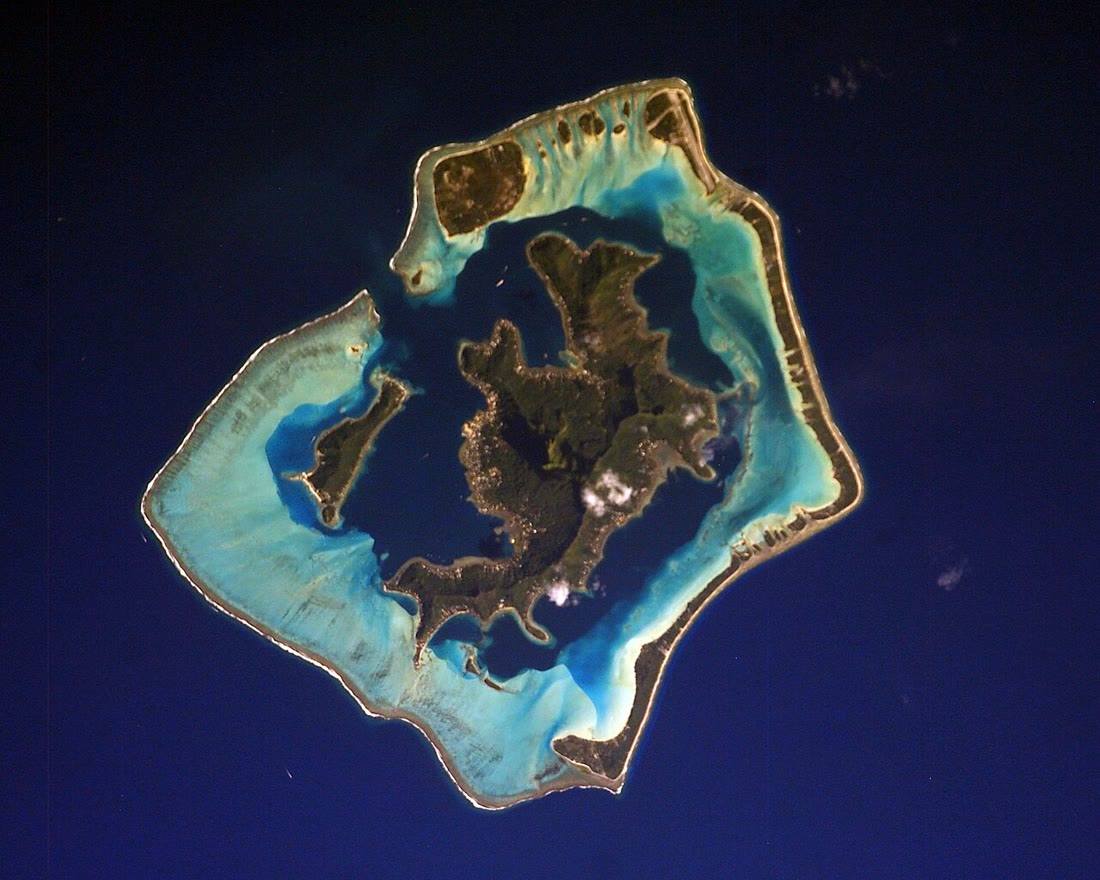
\includegraphics[height=6.9cm]{images/book3/b1-bora-bora.jpg}};
\end{tikzpicture}

{\small Left: the three kinds of coral \omterm{def:b1:chemical-biogenic-sediments:reef}{reef} in cross-section (schematic,
vertical scale much exaggerated), drawn as Darwin explained them: (a)~a \omterm{def:b1:chemical-biogenic-sediments:reef}{reef}
fringing a volcanic island; (b)~the island has sunk and the \omterm{def:b1:chemical-biogenic-sediments:reef}{reef}, growing
upward, has become a barrier separated from the shore by a lagoon; (c)~the
island has sunk out of sight and the \omterm{def:b1:chemical-biogenic-sediments:reef}{reef} is an atoll around a lagoon floored
with carbonate sediment. Right: Bora Bora, a volcanic island in a lagoon
enclosed by a barrier \omterm{def:b1:chemical-biogenic-sediments:reef}{reef} with low islands on it, photographed by an astronaut
from the International Space Station on 19 March 2003 (NASA, public domain, via
Wikimedia Commons).}
\label{fig:b1:chemical-biogenic-sediments:reefs}
\end{omfigure}
% ledger: darwin:reefs, commons:bora-bora

\begin{history}[Reefs on sinking foundations, 1837--1842]
In the course of the voyage of the \emph{Beagle}, Charles Darwin sailed among
the \omterm{def:b1:chemical-biogenic-sediments:reef}{reefs} of the Pacific and Indian Oceans. He reasoned from one fact: reef-building corals, he concluded, do not in ordinary
cases flourish deeper than between 20 and 30 fathoms, about 37 to \qty{55}{m}.
Yet barrier \omterm{def:b1:chemical-biogenic-sediments:reef}{reefs} and atolls rise from deep water, far below that limit. Their
foundations, he argued, must have sunk, slowly enough for the corals to keep
their tops at the surface by growing upward: a \omterm{def:b1:chemical-biogenic-sediments:reef}{reef} that fringes a volcanic
island becomes a barrier as the island sinks inside it, and an atoll when the
island has disappeared. He read his theory before the Geological Society of
London on 31 May 1837 and published it in 1842 in \emph{The Structure and
Distribution of Coral Reefs}, with a map of all the \omterm{def:b1:chemical-biogenic-sediments:reef}{reefs} of the world sorted
into the three kinds. Why ocean islands sink, and how far, is a matter of the
cooling of the plate under them, taken up in the Year~2 volume.
\end{history}
% ledger: darwin:reefs

A \omterm{def:b1:chemical-biogenic-sediments:reef}{reef} survives only if its top stays in the shallow water where its builders
live. Sea level changes, and the foundation may subside; what matters is the
sum of the two, the relative rise of sea level.

\begin{proposition}[Keep up or drown]\label{prop:b1:chemical-biogenic-sediments:keep-up}
Let the top of a \omterm{def:b1:chemical-biogenic-sediments:reef}{reef} lie at the depth $D_0$ below sea level and grow upward at
the rate $a$, while the relative sea level rises at the rate $r$, both
constant. Then the depth of water over the \omterm{def:b1:chemical-biogenic-sediments:reef}{reef} after the time $t$ is
\[
D(t) = D_0 + (r - a)\,t .
\]
If $a \ge r$, the \omterm{def:b1:chemical-biogenic-sediments:reef}{reef} keeps up with the sea (when $a > r$ its top reaches the
surface, and from then on it can only grow sideways); if $a < r$ it falls
behind, and if its builders cannot live deeper than $D_{\max}$, it drowns after
the time $(D_{\max} - D_0)/(r - a)$.
\end{proposition}

\begin{proof}
Measure heights upward from a fixed mark on the foundation. The top of the \omterm{def:b1:chemical-biogenic-sediments:reef}{reef}
is at $h_0 + a t$ and the sea surface at $s_0 + r t$, so the depth of water over
the top is $D = (s_0 - h_0) + (r - a)t = D_0 + (r-a)t$. When $a > r$, $D$
reaches zero at $t = D_0/(a-r)$ and the \omterm{def:b1:chemical-biogenic-sediments:reef}{reef} cannot grow above the sea. When
$a < r$, $D$ grows linearly and reaches $D_{\max}$ when $(r-a)t = D_{\max} -
D_0$.
\end{proof}

A \omterm{def:b1:chemical-biogenic-sediments:reef}{reef} whose top has drowned is not dead at once, but the light dims, the
builders change and the factory slows, so that a \omterm{def:b1:chemical-biogenic-sediments:reef}{reef} that starts to fall
behind falls further: drowned \omterm{def:b1:chemical-biogenic-sediments:reef}{reefs} and platforms, capped by deep-water
sediments, are found on the slopes of many oceanic islands and in the rock
record.

Over millions of years the factories build \omterm{def:b1:chemical-biogenic-sediments:reef}{carbonate platforms}, thick bodies
of shallow-water carbonate that grow as their foundations subside. Two shapes recur
(see the figure below). A \emph{rimmed shelf} has a
flat top, protected behind a rim of \omterm{def:b1:chemical-biogenic-sediments:reef}{reefs} and shoals of \omterm{def:b1:chemical-biogenic-sediments:reef}{ooids} at its edge, which
breaks the waves; behind it lies a quiet lagoon of lime mud, and in front a
steep slope where blocks and debris shed from the rim fall to the basin. A
\emph{ramp} slopes very gently from the shore to the basin without a break: \omterm{def:b1:chemical-biogenic-sediments:reef}{ooid} shoals and shell banks where the waves stir the floor,
then beds of shell debris swept out by storms, then lime mud below the reach of
the waves. A rimmed shelf grows mostly upward and outward from its rim, a ramp
by moving its belts of sediment shoreward or seaward as the sea rises or falls.

\begin{omfigure}
\begin{tikzpicture}[font=\footnotesize, >={Stealth[length=4pt]}]
% (a) rimmed shelf and (b) ramp, schematic cross-sections
\begin{scope}
  \fill[omSea] (0,0.2) rectangle (7.2,2.0);
  \fill[lith limestone, draw=black!60] (0,0) -- (0,1.55) -- (4.3,1.55) -- (4.5,1.75) -- (4.9,1.75) -- (5.1,1.5) -- (6.4,0.35) -- (7.2,0.3) -- (7.2,0) -- cycle;
  \fill[lith reef limestone, draw=black!70] (4.3,1.55) -- (4.5,1.75) -- (4.9,1.75) -- (5.1,1.5) -- (4.8,1.05) -- (4.3,1.05) -- cycle;
  \draw[omSea!60!black] (0,2.0) -- (7.2,2.0);
  \node at (2.1,1.78) {lagoon: lime mud};
  \node[anchor=south, align=center, font=\scriptsize] at (4.7,2.05) {reef rim and\\ ooid shoals};
  \node[anchor=west, font=\scriptsize] at (5.6,1.2) {slope: debris};
  \node[font=\scriptsize] at (6.75,0.75) {basin};
  \node at (3.6,-0.35) {(a) rimmed shelf};
\end{scope}
\begin{scope}[xshift=8.0cm]
  \fill[omSea] (0,0.2) rectangle (7.2,2.0);
  \fill[lith limestone, draw=black!60] (0,0) -- (0,1.85) -- (7.2,0.55) -- (7.2,0) -- cycle;
  \draw[omSea!60!black] (0,2.0) -- (7.2,2.0);
  \draw[densely dashed, black!50] (0,1.6) -- (7.2,1.6) node[pos=1, anchor=south east, font=\scriptsize, inner sep=1pt] {fair-weather waves reach};
  \draw[densely dashed, black!50] (0,1.0) -- (7.2,1.0) node[pos=1, anchor=south east, font=\scriptsize, inner sep=1pt] {storm waves reach};
  \node[anchor=south, font=\scriptsize] at (0.9,2.05) {ooid shoals};
  \node[anchor=south, font=\scriptsize] at (3.4,2.05) {storm shell beds};
  \node[anchor=south, font=\scriptsize] at (6.1,2.05) {lime mud};
  \node at (3.6,-0.35) {(b) ramp};
\end{scope}
\end{tikzpicture}

{\small The two shapes of \omterm{def:b1:chemical-biogenic-sediments:reef}{carbonate platform} (schematic, slopes much
exaggerated). (a)~A rimmed shelf: a rim of \omterm{def:b1:chemical-biogenic-sediments:reef}{reefs} and \omterm{def:b1:chemical-biogenic-sediments:reef}{ooid} shoals breaks the
waves, a quiet lagoon of lime mud lies behind it, and debris shed from the rim
falls down the slope to the basin. (b)~A ramp slopes gently from the shore to
the basin, its sediments sorted by the depth the waves reach.}
\label{fig:b1:chemical-biogenic-sediments:platforms}
\end{omfigure}

\section{Pelagic oozes and the carbonate compensation depth}\label{sec:b1:chemical-biogenic-sediments:oozes}

Far from land, the sea floor receives almost nothing from the continents but
the finest windblown dust. What falls on it instead are the skeletons of the
plankton that lived in the sunlit water kilometres above: the calcite plates of
coccolithophores and the shells of foraminifera, the opal frustules of diatoms
and the skeletons of radiolarians
(pictured a little further on). The long rain of coccoliths
to the sea floor is the main process that makes chalk and much of the
world's limestone.
% ledger: nasa:coccoliths-b3, og:carbonates

\begin{definition}[Calcareous ooze, siliceous ooze]\label{def:b1:chemical-biogenic-sediments:ooze}
An ooze is a fine-grained pelagic sediment, laid down in the open ocean, made
mostly of the skeletons of plankton. It is a \emph{calcareous
ooze}\index{calcareous ooze} when they are of calcium carbonate, chiefly
coccoliths and foraminifera, and a \emph{siliceous ooze}\index{siliceous ooze}
when they are of opal, hydrated amorphous silica, chiefly diatoms and
radiolarians.
\end{definition}
% ledger: og:carbonates

\omterm{def:b1:chemical-biogenic-sediments:ooze}{Calcareous oozes} cover about half of the world's sea floor, but only above a
certain depth: below about \qty{4500}{m} they disappear. The shells do not stop
falling there; they dissolve. The deep ocean is cold and the pressure is high,
and the solubility of calcite increases with depth, mainly because of the
pressure, while the concentration of carbonate ion in the water generally
decreases with depth (the chemistry of these equilibria is recalled from the
chemistry books). Below a certain depth deep water is undersaturated in calcite,
and the shells that reach the floor dissolve faster the deeper they lie.
% ledger: britannica:ccd, slotnick:ccd-definitions

\begin{omfigure}
\begin{tikzpicture}
\node[inner sep=0] (a) at (0,0) {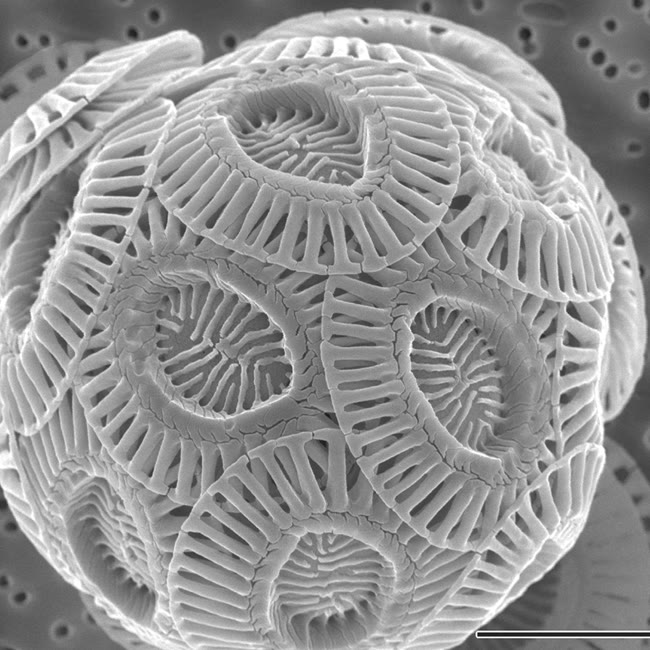
\includegraphics[height=4.3cm]{images/book3/b1-coccolithophore.jpg}};
\node[inner sep=0, anchor=west] (b) at ([xshift=0.25cm]a.east) {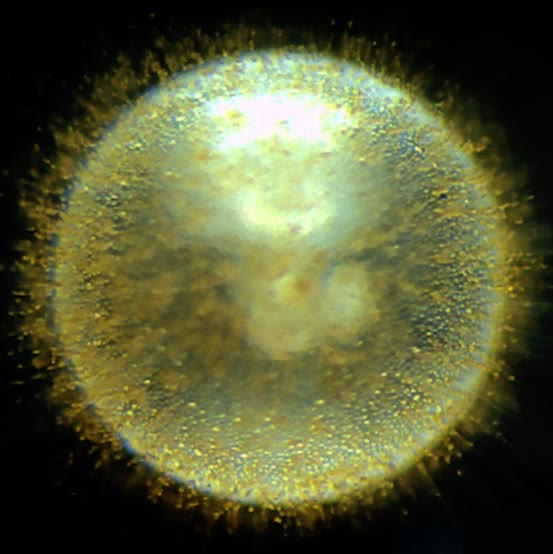
\includegraphics[height=4.3cm]{images/book3/b1-orbulina.jpg}};
\node[inner sep=0, anchor=west] (c) at ([xshift=0.25cm]b.east) {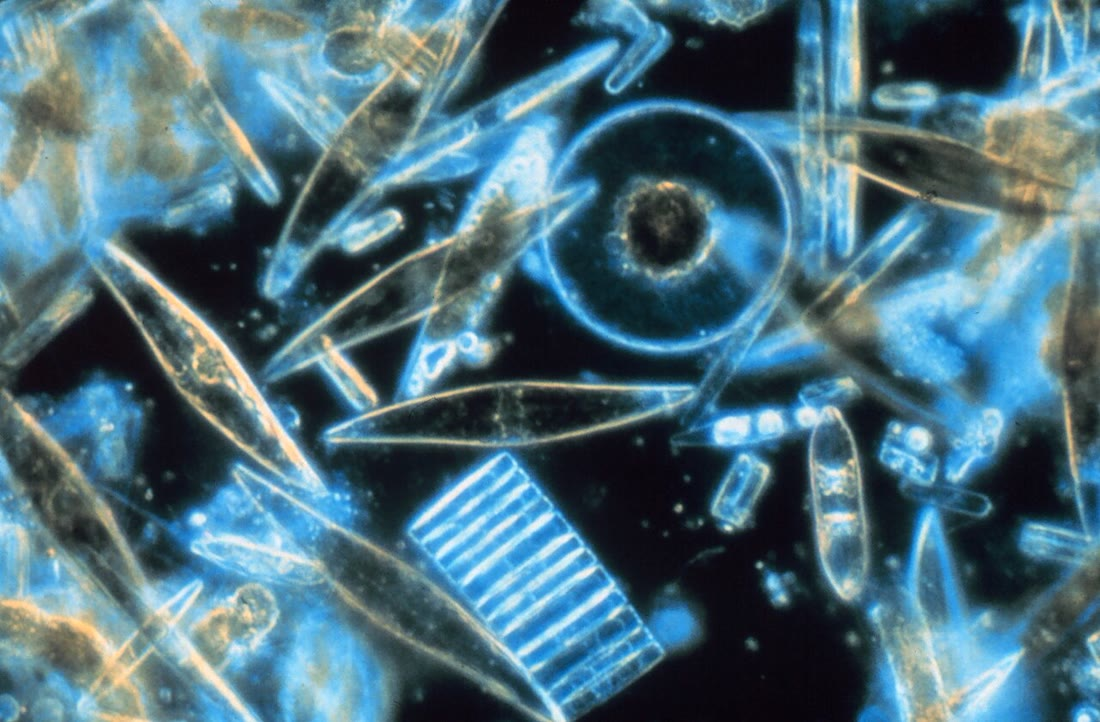
\includegraphics[height=4.3cm]{images/book3/b1-diatoms.jpg}};
\node[font=\footnotesize, anchor=north] at (a.south) {(a) a coccolithophore};
\node[font=\footnotesize, anchor=north] at (b.south) {(b) a foraminifer};
\node[font=\footnotesize, anchor=north] at (c.south) {(c) diatoms};
\end{tikzpicture}

{\small The makers of oozes. (a)~A single cell of \emph{Emiliania huxleyi}
armoured with coccoliths, its plates of calcite (scanning electron microscope;
Alison R.~Taylor, University of North Carolina Wilmington, CC~BY~2.5, via
Wikimedia Commons). (b)~A living planktonic foraminifer, \emph{Orbulina
universa}, its calcite shell surrounded by spines (light microscope; H.~Takagi
and co-authors, 2019, CC~BY~4.0, via Wikimedia Commons). (c)~Living diatoms
from the sea ice of McMurdo Sound, Antarctica, each in its frustule of opal
(light microscope; Gordon T.~Taylor, Stony Brook University, NOAA, public
domain, via Wikimedia Commons).}
\label{fig:b1:chemical-biogenic-sediments:plankton}
\end{omfigure}
% ledger: commons:ehux, commons:orbulina, commons:diatoms-noaa

\begin{definition}[Lysocline, carbonate compensation depth]\label{def:b1:chemical-biogenic-sediments:ccd}
The \emph{lysocline}\index{lysocline} is the depth in the ocean below which the
dissolution of calcite on the sea floor first becomes apparent in the sediment
and its rate increases sharply. The \emph{carbonate compensation
depth}\index{carbonate compensation depth} (CCD) is the depth at which the rate
of dissolution of calcite equals the rate at which calcite rains on the sea
floor; below it no calcium carbonate accumulates. In practice it is placed where
the calcium carbonate content of the surface sediment falls below \qty{10}{\%}
by weight.
\end{definition}
% ledger: slotnick:ccd-definitions

The CCD lies generally hundreds of metres below the \omterm{def:b1:chemical-biogenic-sediments:ccd}{lysocline}. It is not a
fixed level: it is set by a balance between supply and dissolution, so it lies
deeper where the plankton produce more carbonate and where the deep water is
less corrosive. In the Atlantic it lies about \qty{500}{m} deeper than in the
Pacific, the result of both a higher supply of carbonate and a slower
dissolution; within
the western Pacific alone it lies at about \qty{4000}{m} in the north-west and
at about \qty{5100}{m} in the central Pacific. Aragonite, more soluble than
calcite, dissolves at shallower depths still. Over geological time changes in
the supply, in productivity and in dissolution have moved the CCD by more than
\qty{2000}{m}.
% ledger: slotnick:ccd-definitions, britannica:ccd, zhang:ccd-west-pacific

\begin{method}[Locating the lysocline and the CCD]\label{met:b1:chemical-biogenic-sediments:ccd}
\begin{enumerate}
  \item Collect the top few centimetres of sediment at sites of different depths
        in one region, far enough from land and from upwelling for dilution by
        clay or by opal to be small.
  \item Measure the weight per cent of \ce{CaCO3} of each sample and plot it
        against the water depth.
  \item The \omterm{def:b1:chemical-biogenic-sediments:ccd}{lysocline} is the depth where the content starts to fall steeply,
        and where the shells show the first signs of dissolution (broken,
        etched foraminifera).
  \item The CCD is the depth where the content falls to \qty{10}{\%}: read it
        by linear interpolation between the two samples on either side.
\end{enumerate}
\end{method}

On the flank of a mid-ocean ridge, the sea floor is young and shallow near the
axis and sinks as it ages and moves away. A piece of floor born above the CCD
collects \omterm{def:b1:chemical-biogenic-sediments:ooze}{calcareous ooze} until it sinks below the CCD; from then on it receives
only what does not dissolve: the dust that settles from the air above, iron and
manganese oxides, the teeth of fish. This slow, brown deposit is the red clay
of the deep basins.

\begin{proposition}[Crossing the CCD]\label{prop:b1:chemical-biogenic-sediments:flank}
Let the sea floor of age $t$ lie at the depth $d(t) = d_r + C\sqrt t$
(\cref{thm:b1:rifts-ridges-margins:depth-age}), with a ridge axis at the depth $d_r$
shallower than a \omterm{def:b1:chemical-biogenic-sediments:ccd}{carbonate compensation depth} $z_c$ that stays constant. Then
the floor passes below the CCD at the age
\[
t_c = \left(\frac{z_c - d_r}{C}\right)^2 ,
\]
and a site of age $t > t_c$ carries, from the bottom up, the volcanic \omterm{def:b1:layered-earth:layers}{crust},
\omterm{def:b1:chemical-biogenic-sediments:ooze}{calcareous ooze} laid down during the time $t_c$, and red clay laid down during
the time $t - t_c$.
\end{proposition}

\begin{proof}
The depth $d(t)$ increases with $t$, and $d(t_c) = z_c$ gives $C\sqrt{t_c} =
z_c - d_r$, hence $t_c$. Before $t_c$ the floor lies above the CCD, where
calcite rains faster than it dissolves and ooze accumulates; after $t_c$ it
lies below, where no carbonate accumulates and only the insoluble clay is
added. The ooze, once buried under clay, is protected from the corrosive water
above, so the order of the layers is that of the times.
\end{proof}

With $d = 2500 + 350\sqrt t$ (metres, $t$ in millions of years), a CCD at
\qty{4500}{m} is crossed at the age $(2000/350)^2 = \qty{32.7}{Myr}$; at a
half-spreading rate of \qty{25}{mm} a year that is \qty{816}{km} from the axis
(figure below). Drilling into old ocean
floor finds this order again and again: basalt, then \omterm{def:b1:chemical-biogenic-sediments:ooze}{calcareous ooze} or chalk,
then red clay, a record of the floor's journey down the flank. Where the plate
has since moved under a belt of high productivity, near the equator, the clay
can be capped by a new layer of ooze, which is how cores record the motion of
the plates as well as the depth of the CCD.
% ledger: parsons:plate-model

\begin{omfigure}
\begin{tikzpicture}[font=\footnotesize]
\begin{axis}[width=11cm, height=5.6cm, xmin=0, xmax=1750, ymin=2000, ymax=6200, y dir=reverse,
    xlabel={distance from the ridge axis (km), half-spreading rate \qty{25}{mm.yr^{-1}}},
    ylabel={depth (m)}, ytick={2000,3000,...,6000},
    axis on top, clip=false]
  % sea water above the floor
  \addplot[fill=omSea, draw=none] table[x=x_km, y=depth] {figdata/out/bachelor-1-ccd_flank-profile.dat} -- (axis cs:1750,2000) -- (axis cs:0,2000) -- cycle;
  % floor: ooze-covered above the CCD, red clay below
  \addplot[very thick, draw=omLithLime!70!black, restrict x to domain=0:816.3] table[x=x_km, y=depth] {figdata/out/bachelor-1-ccd_flank-profile.dat};
  \addplot[very thick, draw=brown!70!black, restrict x to domain=816.3:1750] table[x=x_km, y=depth] {figdata/out/bachelor-1-ccd_flank-profile.dat};
  \draw[thick, omThm, densely dashed] (axis cs:0,4500) -- (axis cs:1750,4500) node[pos=0.99, anchor=north east, inner sep=1.5pt] {CCD, \qty{4500}{m}};
  \draw[black!60, dotted, thick] (axis cs:0,4050) -- (axis cs:1750,4050) node[pos=0.99, anchor=south east, inner sep=1.5pt] {lysocline (schematic)};
  \fill[omThm] (axis cs:816.3,4500) circle[radius=2pt];
  \node[anchor=north east, align=right] at (axis cs:790,4620) {floor crosses the CCD\\ at \qty{32.7}{Myr}, \qty{816}{km}};
  \node[anchor=north, align=center, omLithLime!40!black] at (axis cs:520,2750) {calcareous ooze\\ accumulates};
  \node[anchor=north west, align=left, brown!60!black] at (axis cs:1000,5180) {red clay over\\ buried ooze};
\end{axis}
% sediment column at the site 1500 km from the axis (60 Myr), schematic
\begin{scope}[xshift=10.6cm, yshift=0.4cm]
  \draw[lith basalt] (0,0) rectangle (0.9,1.0);
  \draw[lith limestone] (0,1.0) rectangle (0.9,2.6);
  \fill[brown!45, draw=black!60] (0,2.6) rectangle (0.9,3.2);
  \node[anchor=west, align=left, font=\scriptsize] at (1.0,0.5) {basaltic crust};
  \node[anchor=west, align=left, font=\scriptsize] at (1.0,1.8) {calcareous ooze\\ (0 to \qty{32.7}{Myr})};
  \node[anchor=west, align=left, font=\scriptsize] at (1.0,2.9) {red clay};
  \node[anchor=south, font=\scriptsize, align=center] at (0.9,3.3) {column at \qty{1500}{km}\\ (schematic)};
\end{scope}
\end{tikzpicture}

{\small Pelagic sediments on a ridge flank. The floor deepens with age by the
\omterm{thm:b1:rifts-ridges-margins:depth-age}{depth--age law} $d = 2500 + 350\sqrt t$ and moves away from the axis at
\qty{25}{mm} a year; above the \omterm{def:b1:chemical-biogenic-sediments:ccd}{carbonate compensation depth}, taken here at
\qty{4500}{m}, it collects \omterm{def:b1:chemical-biogenic-sediments:ooze}{calcareous ooze}, below it only red clay. A site far
from the axis carries basalt, ooze and red clay, from the bottom up (column on
the right, thicknesses schematic). The \omterm{def:b1:chemical-biogenic-sediments:ccd}{lysocline}, drawn a few hundred metres
above the CCD, marks where dissolution begins to show.}
\label{fig:b1:chemical-biogenic-sediments:flank}
\end{omfigure}
% computed in figdata/bachelor-1/ccd_flank.py; ledger: parsons:plate-model, britannica:ccd, slotnick:ccd-definitions

\section{Siliceous oozes and cherts}\label{sec:b1:chemical-biogenic-sediments:silica}

Diatoms, single-celled algae of the plankton, and radiolarians, single-celled
members of the zooplankton, build their skeletons of opal, which they take from
the silicic acid dissolved in seawater. Unlike the calcite of the surface ocean,
the opal is not protected by supersaturation: seawater is undersaturated in it
at all depths, and most of the opal dissolves as soon as the organism dies,
first in the water as it sinks and then on the sea floor. Of the 255~teramoles
of silicon built into opal each year by the plankton of the world ocean, only
about 9.2 are buried in the sediment for good: a preservation of
\qty{3.6}{\%}. A silicon atom brought to the sea by a river is taken up and
released again by the plankton some sixteen times before it is buried, and it
stays about \num{8000} years in the ocean.
% ledger: treguer:silica

So \omterm{def:b1:chemical-biogenic-sediments:ooze}{siliceous oozes} form where the production of opal is so high that even
\qty{3.6}{\%} of it adds up, and where little else dilutes it: around the
Southern Ocean, in the North Pacific, along the equator in the Pacific and on
continental margins, the places where deep water rich in nutrients rises to
the surface (\cref{ch:b1:ocean-circulation}). They also dominate below the CCD
under productive waters, where the calcite that fell with them has dissolved.
% ledger: treguer:silica, og:carbonates

\begin{definition}[Chert]\label{def:b1:chemical-biogenic-sediments:chert}
A \emph{chert}\index{chert} is a hard, dense sedimentary rock of
microcrystalline quartz, formed in most cases from biogenic opal that dissolved
and recrystallised after burial; it occurs as beds, often from \omterm{def:b1:chemical-biogenic-sediments:ooze}{siliceous oozes},
or as nodules, of which flint, in chalk, is the best known.
\end{definition}
% ledger: og:carbonates

A diatom ooze that has not been recrystallised becomes diatomite, a light,
white, porous rock, almost pure opal. With burial and time the opal turns into
other forms of silica and finally into quartz, and the silica migrates: it
leaves the chalk, for instance, and gathers in nodules of flint along certain
beds. How this happens belongs to diagenesis (\cref{ch:b1:diagenesis-basins}).

\section{Evaporites}\label{sec:b1:chemical-biogenic-sediments:evaporites}

Where a body of seawater loses more water by evaporation than it receives, its
salts concentrate until they precipitate one after another. The composition of
seawater is the same, in its major ions, in all the oceans
(\cref{tab:b1:chemical-biogenic-sediments:seawater}).

\begin{table}[htbp]
\centering\small
\begin{tabular}{@{}lrrr@{}}
\hline
ion & mass fraction of sea salt & \si{g} per \si{kg} of seawater & \si{mmol} per \si{kg} \\
\hline
chloride \ce{Cl-} & 0.5503 & 19.353 & 545.9 \\
sodium \ce{Na+} & 0.3066 & 10.781 & 469.0 \\
sulfate \ce{SO4^2-} & 0.0771 & 2.712 & 28.2 \\
magnesium \ce{Mg^2+} & 0.0365 & 1.284 & 52.8 \\
calcium \ce{Ca^2+} & 0.0117 & 0.412 & 10.3 \\
potassium \ce{K+} & 0.0113 & 0.399 & 10.2 \\
hydrogen carbonate \ce{HCO3-} & 0.0030 & 0.105 & 1.72 \\
bromide \ce{Br-} & 0.0019 & 0.067 & 0.84 \\
\hline
all solutes & 1 & 35.165 & \\
\hline
\end{tabular}
\caption{The major ions of seawater of the reference composition, for a
salinity of \qty{35.165}{g} of salt per kilogram of seawater. Chloride and
sodium make \qty{86}{\%} of the salt by mass; carbonate, strontium, borate and
fluoride make up most of the remainder.}
\label{tab:b1:chemical-biogenic-sediments:seawater}
\end{table}
% ledger: teos10:reference-composition, teos10:reference-salinity (g and mmol computed in evaporation.py)

\begin{definition}[Evaporite, evaporation sequence, sabkha]\label{def:b1:chemical-biogenic-sediments:evaporite}
An \emph{evaporite}\index{evaporite} is a sediment or sedimentary rock of salts
precipitated from a natural brine concentrated by evaporation: chiefly gypsum
\ce{CaSO4.2H2O} and anhydrite \ce{CaSO4}, halite \ce{NaCl}, and the potassium and
magnesium salts. The \emph{evaporation sequence}\index{evaporation sequence} is
the order in which the \omterm{def:b1:rock-forming-minerals:mineral}{minerals} precipitate from evaporating seawater, the least
soluble first: calcium carbonate, then gypsum, then halite, then the potassium
and magnesium salts. A \emph{sabkha}\index{sabkha} is a coastal salt flat, at or
just above the level of the highest tides, where gypsum, anhydrite and halite
grow within the sediment from the evaporating brine that soaks it.
\end{definition}
% ledger: og:carbonates, warren:brine-stages

The sequence was watched as early as 1849 by Usiglio, who evaporated a vessel
of seawater to dryness; the most precise measurements come from the salt
works of Great Inagua in the Bahamas, where seawater is led through a series of
ponds of increasing concentration. Calcium carbonate begins to precipitate when
the brine is 1.8~times as concentrated as seawater, gypsum at 3.8~times, halite
at 10.6~times; in the laboratory magnesium sulfate followed at about 70~times
and potassium salts above 90~times. Since the salts precipitated before are a
negligible part of the mass, a concentration factor of 10.6 means that
$1/10.6$, about \qty{9}{\%}, of the water is left: halite comes only when nine
tenths of the water have gone (figure below, panel~a).
The brine grows denser as it concentrates, from \qty{1.03}{g.cm^{-3}} for
seawater to about \num{1.13} when gypsum forms, \num{1.22} with halite and more
than \num{1.30} with the bittern salts, the last salts of all.
% ledger: warren:brine-stages, mccaffrey:thresholds

How much of each salt a kilogram of seawater can give follows from
\cref{tab:b1:chemical-biogenic-sediments:seawater} by counting the ion that runs
out first. Calcium carbonate is limited by the carbonate and hydrogen carbonate,
\qty{1.10}{mmol}, about \qty{0.11}{g}. Gypsum takes the remaining calcium,
\qty{9.18}{mmol}, \qty{1.58}{g}, sulfate being in excess. Halite takes all the
sodium, \qty{469}{mmol}, \qty{27.4}{g}, chloride being in excess. What is left,
about \qty{6.3}{g} of magnesium, potassium, sulfate, chloride and bromide, makes
the bittern salts. Halite is \qty{78}{\%} of the whole: an \omterm{def:b1:chemical-biogenic-sediments:evaporite}{evaporite} basin
dried out is above all a mass of rock salt.
% computed in figdata/bachelor-1/evaporation.py; ledger: teos10:reference-composition, mccaffrey:thresholds

\begin{omfigure}
\begin{tikzpicture}[font=\footnotesize]
\begin{axis}[name=a, width=7.6cm, height=5.6cm, xmode=log, xmin=1, xmax=100, ymin=0, ymax=1.05,
    xlabel={concentration factor of the brine}, ylabel={fraction of the water left},
    title={\footnotesize (a) onsets of the evaporation sequence}, grid=major, grid style={black!10},
    log ticks with fixed point]
  \addplot[omDef, thick] table[x=CF, y=f_left] {figdata/out/bachelor-1-evaporation-curve.dat};
  \addplot[omThm, only marks, mark=*, mark size=1.8pt] table[x=CF, y=f_left] {figdata/out/bachelor-1-evaporation-steps.dat};
  \node[anchor=south west, font=\scriptsize] at (axis cs:1.8,0.556) {\ce{CaCO3} (1.8)};
  \node[anchor=south west, font=\scriptsize] at (axis cs:3.8,0.263) {gypsum (3.8)};
  \node[anchor=south west, font=\scriptsize] at (axis cs:10.6,0.094) {halite (10.6)};
  \node[anchor=south, font=\scriptsize, align=center] at (axis cs:60,0.16) {Mg, K salts\\ (70, 90)};
\end{axis}
\begin{axis}[at={(a.east)}, anchor=west, xshift=1.7cm, width=7.0cm, height=5.6cm,
    ybar, bar width=14pt, ymin=0, ymax=32, xmin=0.4, xmax=4.6,
    xtick={1,2,3,4}, xticklabels={\ce{CaCO3}, gypsum, halite, bittern},
    ylabel={grams per kg of seawater}, title={\footnotesize (b) masses laid down},
    nodes near coords, nodes near coords style={font=\scriptsize, /pgf/number format/precision=2},
    every node near coord/.append style={/pgf/number format/fixed}]
  \addplot[fill=omDef!40, draw=omDef] table[x=idx, y=g_per_kg] {figdata/out/bachelor-1-evaporation-masses.dat};
\end{axis}
\end{tikzpicture}

{\small The evaporation of seawater. (a)~The fraction of the water left when the
brine is concentrated by a given factor, with the onset of each \omterm{def:b1:rock-forming-minerals:mineral}{mineral}
measured at the salt works of Great Inagua and in the laboratory (McCaffrey,
Lazar and Holland, 1987). (b)~The masses laid down per kilogram of seawater
evaporated to dryness, each \omterm{def:b1:rock-forming-minerals:mineral}{mineral} taking all of the ion that limits it
(gypsum counted with its water; the bittern salts counted without theirs),
computed from the reference composition of seawater.}
\label{fig:b1:chemical-biogenic-sediments:evaporation}
\end{omfigure}
% computed in figdata/bachelor-1/evaporation.py; ledger: mccaffrey:thresholds, teos10:reference-composition

From these masses the thickness of salt that a given body of water can leave
follows at once.

\begin{proposition}[Salt from a column of seawater]\label{prop:b1:chemical-biogenic-sediments:column}
A column of seawater of height $H$ and density $\rho_{sw}$, evaporated to
dryness, lays down a layer of a \omterm{def:b1:rock-forming-minerals:mineral}{mineral} of density $\rho_x$ whose thickness is
\[
h_x = \frac{\rho_{sw}\,H\,m_x}{\rho_x},
\]
where $m_x$ is the mass of that \omterm{def:b1:rock-forming-minerals:mineral}{mineral} laid down per unit mass of seawater.
\end{proposition}

\begin{proof}
A unit area of the column holds the mass $\rho_{sw}H$ of seawater, which lays
down the mass $\rho_{sw}Hm_x$ of the \omterm{def:b1:rock-forming-minerals:mineral}{mineral}. Spread over the same unit area as
a layer of density $\rho_x$, it has the thickness $\rho_{sw}Hm_x/\rho_x$.
\end{proof}

With $\rho_{sw} = \qty{1030}{kg.m^{-3}}$, $m = \qty{27.4}{g.kg^{-1}}$ and the
density of halite, \qty{2170}{kg.m^{-3}}, a column of seawater \qty{1000}{m} high
leaves \qty{13.0}{m} of halite; with gypsum, of density \qty{2300}{kg.m^{-3}}, it
leaves \qty{0.71}{m} of gypsum. This is the thickness problem of \omterm{def:b1:chemical-biogenic-sediments:evaporite}{evaporites}:
salt beds hundreds of metres or kilometres thick cannot be the residue of a
single filling of any basin, however deep.
% computed in figdata/bachelor-1/evaporation.py; ledger: warren:brine-stages, webmineral:evaporites

The answer is a basin that keeps receiving seawater. A basin separated from the
ocean by a sill, a shallow strait or a barrier, in a dry climate, loses water by
evaporation over its whole area; seawater flows in over the sill to replace it,
bringing new salt, and the denser brine may flow out at depth over the sill
(figure below). The concentration of the brine
is set by the balance of these flows.

\begin{proposition}[The barred basin]\label{prop:b1:chemical-biogenic-sediments:barred}
Let a well-mixed basin of area $A$ lose the volume $EA$ of water per unit time
by net evaporation, receive seawater at the volume rate $Q_{\mathrm{in}}$ and
return brine to the ocean at the volume rate $Q_{\mathrm{out}}$, in a steady
state. For an ion that does not precipitate, the brine is concentrated by the
factor
\[
k = \frac{Q_{\mathrm{in}}}{Q_{\mathrm{out}}} = \frac{Q_{\mathrm{in}}}{Q_{\mathrm{in}} - EA}
\]
with respect to seawater (the volumes counted as if of equal density).
\end{proposition}

\begin{proof}
In a steady state the volume of the basin does not change, so the inflow
balances the outflow and the evaporation: $Q_{\mathrm{in}} = Q_{\mathrm{out}} +
EA$. The ion enters at the concentration $c_0$ of seawater and leaves only with
the brine, at its concentration $c$; since it does not precipitate, its mass in
the basin is steady when $Q_{\mathrm{in}}c_0 = Q_{\mathrm{out}}c$. Hence $c/c_0 =
Q_{\mathrm{in}}/Q_{\mathrm{out}}$, and substituting $Q_{\mathrm{out}}$ gives the
second form.
\end{proof}

The outflow controls what the basin lays down. If more than a tenth of the
inflow returns to the ocean as brine, $k$ stays below 10.6 and the basin lays
down carbonate and gypsum but never halite; if the outflow is smaller, the
brine reaches halite saturation and the basin fills with salt; if the strait is
closed altogether, the basin dries out and its level falls at the rate $E$.

\begin{omfigure}
\begin{tikzpicture}[font=\footnotesize, >={Stealth[length=4pt]}]
% barred evaporite basin (schematic)
\fill[omSea] (0,1.0) rectangle (3.2,3.0);
\fill[omSea!70!yellow!40] (3.6,0.6) rectangle (11.2,3.0);
\fill[omSea] (3.0,2.45) rectangle (3.8,3.0);
\draw[lith shale] (0,0) -- (0,1.0) -- (2.6,1.0) -- (3.2,2.4) -- (3.6,2.45) -- (4.4,0.6) -- (10.2,0.6) -- (11.2,2.2) -- (11.2,0) -- cycle;
\draw[lith evaporite] (4.25,0.95) -- (4.4,0.6) -- (10.2,0.6) -- (10.41,0.95) -- cycle;
\fill[omLithGranite!50, draw=black!50] (5.6,0.95) rectangle (9.0,1.35);
\draw[omSea!60!black] (0,3.0) -- (11.2,3.0);
\draw[->, thick, omDef] (1.6,2.75) -- (4.6,2.75) node[right] {inflow of seawater};
\draw[->, thick, omThm, densely dashed] (4.6,1.5) .. controls (4.1,2.35) and (3.8,2.57) .. (3.1,2.57) .. controls (2.6,2.57) and (2.3,2.2) .. (2.1,1.7) node[anchor=north east, inner sep=1pt] {outflow of brine};
\foreach \x in {6.0,7.4,8.8,10.2} {\draw[->, black!60] (\x,3.1) -- (\x,3.7);}
\node[anchor=south] at (8.1,3.7) {evaporation over the basin};
\node at (0.8,2.15) {ocean};
\node[anchor=south] at (3.4,3.0) {sill};
\node[anchor=north, fill=white, inner sep=1pt] at (7.3,0.55) {gypsum and anhydrite};
\node at (7.3,1.15) {halite};
\node at (7.3,2.2) {dense brine};
\end{tikzpicture}

{\small A barred \omterm{def:b1:chemical-biogenic-sediments:evaporite}{evaporite} basin (schematic): seawater flows in over a sill to
replace the water evaporated from the basin; the dense brine sinks and part of
it flows back to the ocean at depth. The smaller the outflow, the more
concentrated the brine; here it has passed halite saturation and halite lies
over the earlier gypsum.}
\label{fig:b1:chemical-biogenic-sediments:barred}
\end{omfigure}

The largest young \omterm{def:b1:chemical-biogenic-sediments:evaporite}{evaporite} of the world lies under the floor of the
Mediterranean. Between 5.97 and 5.33~million years ago, in the Messinian age, the
exchanges of water between the Mediterranean and the Atlantic were restricted,
and \omterm{def:b1:chemical-biogenic-sediments:evaporite}{evaporites} up to \qty{2}{km} thick were laid down in the deep basins, their
halite mostly in a short interval between 5.60 and 5.55~million years ago. How
it happened is still debated. In one model the sea was largely cut off and its
level fell by about \qty{1500}{m}, the deep basins becoming salt lakes and the
rivers cutting deep canyons into the dry margins; in others the basin stayed
connected and full, a barred basin on a vast scale. Both must explain
kilometres of salt, which one filling of the sea could never give.
% ledger: vasiliev:msc

\section{Exercises}

\begin{exercise}[$\star$]\label{exo:b1:chemical-biogenic-sediments:1}
Seawater of the reference composition holds \qty{35.165}{g} of salt per
kilogram, of which the mass fractions of chloride, sodium, sulfate and magnesium
are 0.5503, 0.3066, 0.0771 and 0.0365. Compute the mass of each ion in a kilogram
of seawater, and the fraction of the salt made of sodium and chloride together.
% ledger: teos10:reference-composition, teos10:reference-salinity
\end{exercise}

\begin{exercise}[$\star$]\label{exo:b1:chemical-biogenic-sediments:2}
Calcium carbonate, gypsum, halite and magnesium sulfate begin to precipitate
from seawater concentrated 1.8, 3.8, 10.6 and 70 times. For each, compute the
fraction of the original water left and the fraction already evaporated.
% ledger: mccaffrey:thresholds
\end{exercise}

\begin{exercise}[$\star$]\label{exo:b1:chemical-biogenic-sediments:3}
On \omterm{def:b1:chemical-biogenic-sediments:reef}{reefs} dominated by \emph{Acropora} the carbonate budget is \qty{8.4}{kg} of
\ce{CaCO3} per square metre and per year and the \omterm{def:b1:chemical-biogenic-sediments:reef}{reef} grows by \qty{4.2}{mm} a
year. (a)~With \cref{prop:b1:chemical-biogenic-sediments:accretion}, compute the
dry bulk density of the \omterm{def:b1:chemical-biogenic-sediments:reef}{reef}. (b)~What is its porosity if its grains are of
aragonite, of density \qty{2.93}{g.cm^{-3}}? of calcite, of density
\qty{2.71}{g.cm^{-3}}? (c)~At the same bulk density, how fast would a \omterm{def:b1:chemical-biogenic-sediments:reef}{reef} with
the average budget of \qty{3.7}{kg.m^{-2}.yr^{-1}} grow?
% ledger: perry:chagos, webmineral:polymorphs, hom:calcite
\end{exercise}

\begin{exercise}[$\star$]\label{exo:b1:chemical-biogenic-sediments:4}
Surface sediments from one region of the ocean floor contain the following
weight per cent of \ce{CaCO3}: 88 at \qty{3000}{m}, 85 at \qty{3500}{m}, 80 at
\qty{4000}{m}, 62 at \qty{4300}{m}, 35 at \qty{4500}{m}, 12 at \qty{4700}{m}, 6
at \qty{4800}{m} and 2 at \qty{5000}{m}. With
\cref{met:b1:chemical-biogenic-sediments:ccd}, locate the \omterm{def:b1:chemical-biogenic-sediments:ccd}{lysocline} and the CCD.
\end{exercise}

\begin{exercise}[$\star\star$]\label{exo:b1:chemical-biogenic-sediments:5}
(a)~Write the balanced equation of the precipitation of calcium carbonate from
calcium and hydrogen carbonate ions, and compute the mass of carbon dioxide
released per kilogram of \ce{CaCO3} laid down (molar masses \qty{100.09}{g.mol^{-1}}
and \qty{44.01}{g.mol^{-1}}). (b)~How much would a \omterm{def:b1:chemical-biogenic-sediments:reef}{reef} with a budget of
\qty{3.7}{kg.m^{-2}.yr^{-1}} release per square metre and per year, by this
equation? (c)~Why does a \omterm{def:b1:chemical-biogenic-sediments:reef}{reef}, which turns dissolved carbon into rock, release
carbon dioxide?
% ledger: perry:chagos
\end{exercise}

\begin{exercise}[$\star\star$]\label{exo:b1:chemical-biogenic-sediments:6}
Take the sea floor at the depth $d = 2500 + 350\sqrt t$ (metres, $t$ in
millions of years), spreading from its ridge at the half-rate \qty{25}{mm} a
year. (a)~At what age and at what distance from the axis does it cross a CCD at
\qty{4500}{m}? (b)~The same for a CCD at \qty{5100}{m}, as in the central
Pacific. (c)~How long would floor \qty{60}{Myr} old have received red clay in
each case?
% ledger: parsons:plate-model, zhang:ccd-west-pacific
\end{exercise}

\begin{exercise}[$\star\star$]\label{exo:b1:chemical-biogenic-sediments:7}
A \omterm{def:b1:chemical-biogenic-sediments:reef}{reef} grows at \qty{4.2}{mm} a year. (a)~Can it keep up with a relative
rise of sea level of \qty{3}{mm} a year? (b)~Its top lies \qty{2}{m} below the
sea when the relative rise becomes \qty{10}{mm} a year. If its builders cannot
live deeper than \qty{50}{m}, how long until it drowns?
(c)~Why may it in fact drown sooner?
% ledger: perry:chagos
\end{exercise}

\begin{exercise}[$\star\star$]\label{exo:b1:chemical-biogenic-sediments:8}
Buried under a few hundred metres of sediment, gypsum \ce{CaSO4.2H2O}
(\qty{172.17}{g.mol^{-1}}, density \qty{2.30}{g.cm^{-3}}) loses its water and
becomes anhydrite \ce{CaSO4} (\qty{136.14}{g.mol^{-1}}, density
\qty{2.97}{g.cm^{-3}}). (a)~Write the reaction. (b)~Compute the molar volumes of
the two \omterm{def:b1:rock-forming-minerals:mineral}{minerals} and the change of volume of the solid. (c)~What fraction of
the mass of the gypsum leaves as water? What can this water do in the rocks
around?
% ledger: webmineral:evaporites
\end{exercise}

\begin{exercise}[$\star\star$]\label{exo:b1:chemical-biogenic-sediments:9}
The plankton of the world ocean build 255~teramoles of silicon into opal a
year, and 9.2 are buried. (a)~Compute the fraction preserved and the fraction
dissolved. (b)~Why can \omterm{def:b1:chemical-biogenic-sediments:ooze}{siliceous ooze} nevertheless form, and where? (c)~Why
is the record of diatoms in the sediment a biased picture of the diatoms that
lived in the water?
% ledger: treguer:silica
\end{exercise}

\begin{exercise}[$\star\star\star$]\label{exo:b1:chemical-biogenic-sediments:10}
A barred basin of area \qty{10000}{km^2} loses by net evaporation \qty{1.5}{m}
of water a year. (a)~Compute the volume evaporated each year. (b)~With
\cref{prop:b1:chemical-biogenic-sediments:barred}, compute the concentration
factor of the brine when the inflow over the sill is \qty{1.8e10}{m^3} a year,
and when it is \qty{1.575e10}{m^3} a year. Which \omterm{def:b1:rock-forming-minerals:mineral}{minerals} can precipitate in
each case? (c)~Up to what inflow does the basin lay down halite?
% ledger: mccaffrey:thresholds
\end{exercise}

\begin{exercise}[$\star\star\star$]\label{exo:b1:chemical-biogenic-sediments:11}
Seawater holds \qty{0.0673}{g} of bromide per kilogram. When halite
precipitates, it takes up bromide in proportion to its concentration in the
brine: the bromide content of the halite is $D = 0.032$ times that of the
brine. (a)~Compute the bromide content of the brine, in milligrams per
kilogram, and of the first halite, when the brine is 10.6~times as concentrated
as seawater. (b)~The same when the brine has reached 30~times. (c)~Bromide is
hardly removed from the brine by the halite: why? (d)~In a thick bed of halite,
the bromide content rises upward, then suddenly falls back. What happened to
the basin?
% ledger: teos10:reference-composition, mccaffrey:dbr, mccaffrey:thresholds
\end{exercise}

\begin{exercise}[$\star\star\star$]\label{exo:b1:chemical-biogenic-sediments:12}
A site on the flank of a ridge has the depth $d = 2500 + 350\sqrt t$ and is now
\qty{70}{Myr} old. Suppose that \omterm{def:b1:chemical-biogenic-sediments:ooze}{calcareous ooze} accumulates at \qty{2}{cm} per
thousand years above the CCD and red clay at \qty{1}{mm} per thousand years
below it, and neglect compaction. (a)~Compute the thickness of ooze and of red
clay at the site for a CCD at \qty{4500}{m}. (b)~The same for a CCD
\qty{500}{m} deeper, as in the Atlantic. (c)~A core at the site shows a thin
layer of ooze within the red clay. Give two possible explanations.
% ledger: parsons:plate-model, britannica:ccd
\end{exercise}

\section{Problem: Salt from a vanished sea}

\begin{problem}[{Weekend problem --- how much seawater it takes to make a salt
basin, and how long}]
\label{pb:b1:chemical-biogenic-sediments:1}
% values: calc/ch22.py; the basin, its area, inflow and evaporation are invented
An inland sea of area $A = \qty{1.0e5}{km^2}$, \qty{1000}{m} deep, is joined to
the ocean by a strait over a shallow sill. Its floor, now buried, carries
\qty{1.5}{km} of halite. Take for seawater the density \qty{1030}{kg.m^{-3}} and
the masses laid down per kilogram computed in the chapter: \qty{0.110}{g} of
\ce{CaCO3}, \qty{1.581}{g} of gypsum, \qty{27.41}{g} of halite and
\qty{6.34}{g} of bittern salts; for the \omterm{def:b1:rock-forming-minerals:mineral}{minerals} the densities: calcite
\qty{2710}{kg.m^{-3}}, gypsum \qty{2300}{kg.m^{-3}}, anhydrite
\qty{2970}{kg.m^{-3}}, halite \qty{2170}{kg.m^{-3}}. Treat the sea as a box with
vertical walls.

\medskip
\noindent\textbf{Part I --- One filling.}
\begin{enumerate}
  \item Compute the mass of seawater above one square metre of the floor, and
        the mass of salt it holds (\qty{35.165}{g.kg^{-1}}).
  \item Compute the mass of gypsum and of halite laid down on one square metre
        when the sea evaporates to dryness.
  \item With \cref{prop:b1:chemical-biogenic-sediments:column}, compute the
        thickness of calcium carbonate, of gypsum and of halite.
  \item Buried, the gypsum becomes anhydrite. What is then the thickness of the
        sulfate layer?
  \item What fraction of the dry salt is halite? Why is a dried-out sea mostly
        rock salt?
  \item In what order, from the bottom up, do the layers lie? Why?
\end{enumerate}

\noindent\textbf{Part II --- The brine as the sea dries.}
\begin{enumerate}[resume]
  \item At what depth of brine, in the box, do calcium carbonate, gypsum and
        halite begin to precipitate?
  \item What fraction of the water has evaporated when halite appears?
  \item Below what depth of brine do the magnesium and potassium salts begin?
  \item How dense is the brine at each stage? What does this mean for a brine
        that meets fresh seawater flowing in?
  \item Why is the first deposit, the carbonate, rarely seen as a separate
        layer in an \omterm{def:b1:chemical-biogenic-sediments:evaporite}{evaporite} basin?
  \item The bromide content of the halite rises from the base to the top of
        the halite layer of one filling. Why?
\end{enumerate}

\noindent\textbf{Part III --- How many fillings?}
\begin{enumerate}[resume]
  \item How many fillings of the basin, evaporated each time to dryness, would
        be needed to lay down the \qty{1.5}{km} of halite?
  \item How much anhydrite would accompany it, and how would it be
        distributed in the section?
  \item How thick would the bittern salts be, if they were all kept, with a
        mean density of \qty{2000}{kg.m^{-3}}? Why are they so often missing?
  \item How would the bromide content of the halite record each refilling?
  \item The Messinian \omterm{def:b1:chemical-biogenic-sediments:evaporite}{evaporites} reach \qty{2}{km}. How many fillings of a
        \qty{1000}{m} sea would their halite need, if they were all halite?
\end{enumerate}

\noindent\textbf{Part IV --- Inflow and time.}
\begin{enumerate}[resume]
  \item Seawater flows in over the sill at \qty{5000}{m^3.s^{-1}} and no brine
        flows out; the level stays constant. Compute the net evaporation rate
        over the sea, in metres a year (a year of $365.25$ days).
  \item Compute the mass of salt that enters the sea each year.
  \item If all its halite is laid down evenly on the floor, how thick a layer
        of halite forms each year?
  \item How long does the \qty{1.5}{km} of halite take to form?
  \item The strait closes. How fast does the level fall, and how long until the
        sea dries out, if the evaporation rate stays the same?
  \item How long after the closure does halite begin to precipitate?
  \item To the nearest whole number, how many fillings of the basin did its
        salt require?
\end{enumerate}
\end{problem}
